% Created 2019-11-15 Fri 14:53
% Intended LaTeX compiler: pdflatex
\documentclass[11pt]{article}
\usepackage[utf8]{inputenc}
\usepackage[T1]{fontenc}
\usepackage{graphicx}
\usepackage{grffile}
\usepackage{longtable}
\usepackage{wrapfig}
\usepackage{rotating}
\usepackage[normalem]{ulem}
\usepackage{amsmath}
\usepackage{textcomp}
\usepackage{amssymb}
\usepackage{capt-of}
\usepackage{hyperref}
\usepackage{minted}
\usepackage[margin=.5in]{geometry}
\author{Guilherme Gomes Haetinger}
\date{\today}
\title{Class Computations}
\hypersetup{
 pdfauthor={Guilherme Gomes Haetinger},
 pdftitle={Class Computations},
 pdfkeywords={},
 pdfsubject={},
 pdfcreator={Emacs 27.0.50 (Org mode 9.2.6)}, 
 pdflang={English}}
\begin{document}

\maketitle
\tableofcontents

\begin{minted}[]{r}
library(ggplot2)
\end{minted}


\section{What's the expected value of a binomial distribution where 25 coins are flipped, each having 30\% chance of heads?}
\label{sec:orgceb31bd}
\begin{minted}[]{r}
mean(rbinom(10000, 25, 0.3))
\end{minted}

\begin{verbatim}
7.4631
\end{verbatim}

\section{Simulate 100,000 flips of a coin with a 40\%/20\% chance of heads}
\label{sec:org3fd55ac}
\begin{minted}[]{r}
A <- rbinom(100000, 1, .4)
B <- rbinom(100000, 1, .2)
mean(A & B)
\end{minted}

\begin{verbatim}
0.08124
\end{verbatim}

\subsection{\(P(A|B) = P(A) + P(B) - P(A \cap B)\)}
\label{sec:orga129314}
\begin{minted}[]{r}
mean(A) + mean(B) - mean(A & B)
\end{minted}

\section{Simulating from the binomial and the normal}
\label{sec:org1fe5802}
\begin{minted}[]{r}
binom_sample <- data.frame(value = rbinom(100000, 1000, .2))
normal_sample <- data.frame(value = rnorm(100000, 200, sqrt(160)))

binom_sample$type = "binom"
normal_sample$type = "normal"

joint <- rbind(binom_sample, normal_sample)

ggplot(joint, aes(value, fill = type)) + geom_histogram()
\end{minted}

\begin{center}
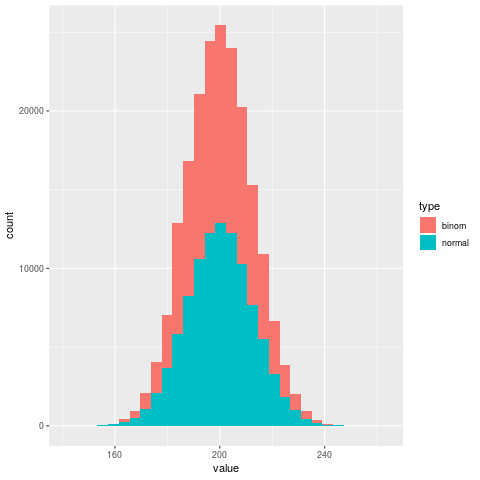
\includegraphics[width=.9\linewidth]{test.png}
\end{center}



\begin{minted}[]{python}
x = 2  
\end{minted}
\end{document}
